\documentclass{article}

\usepackage[utf8]{inputenc}
\usepackage{enumerate}
\usepackage{mathtools}
\usepackage{pgfplots}
\usepackage{tikz} 
\setlength\parindent{0pt}


\title{
    General NP-Hard Solvers \\
    \large applied to the \\
    Travelling Salesman Problem
}

\author{Gary Sun}

\date{}

\begin{document}

\maketitle

\section{Introduction}
\subsection{NP-Hard Problems}
NP-hard (non-deterministic polynomial-time hard) problems are those that are 
\begin{itemize}
    \item verifiable in polynomial time by a deterministic turing machine OR
    \item solvable in polynomial time by a non-deterministic turing machine
\end{itemize}

Due to their difficulty in solving, there tends to be a general algorithms.

\subsection{The Travelling Salesman Problem}
The travelling salesman is an example of an NP-hard combinatorial optimisation problem.

It goes as follows:

Given a weighted graph, starting at a vertex, find the minimal cost to travel to all the vertices of the graph once, before returning back to the starting vertex.
\\
It has many applications, i.e. in

\begin{itemize}
    \item logistics (determining an optimal route of least cost)
    \item the manufacturing of microchips (determining the path of a soldering iron which has to react all contacts.
\end{itemize}

\section{Deterministic Algorithms}

W

\subsection{Brute Force}

Whilst it is the least efficient algorithm to solve this, it is worth going over its procedure.


\subsection{Branch and Bound}

A branch and bound algorithm is one that explores certain candidate solutions a

\section{Non-Deterministic Algorithms}

\subsection{Genetic Algorithm}

\subsection{Simulated Annealing}

Simulated Annealing is a stochastic global search optimisation algorithm.
It can be used to find an approx global minimum or maximum and may be preferred over exact algorithms due to faster runtime.
\\

\subsubsection{Origin}
It is based off annealing in metallurgy, where the structure of the material changes randomly rapidly. when the temperature is high.
As a result, at the beginning, SA may choose a solution, even if does not lead to an improvement in the objective function.

However, overtime as the temperature drops and loses its internal energy, the structure settles into a more stable form.
Hence, as the temperature drops, the SA algorithm will with a higher probability discard solutions that do not improve the objective function, and always choosing those that improve the objective function.

Finally, the resulting material structure reaches its absolute (global) minimum internal energy configuration.
Similarly, the SA algorithm will then find an approximate (or the) solution for maximising the objective function.

Note the temperature and cooling rate has to be carefully selected.
If the temperature cools too fast, then in the process may get stuck at a local minimum. 
This is similar to what happens in a greedy method, where the search gets stuck in a local minimum.
Hence, the introduction of the temperature, and probabilistic acceptance of worse states allows for a higher chance of finding the global minimum.
\\

\subsubsection{Process}

\begin{enumerate}[Step 1:]
    \item Choose a suitable initial temperature $T_0$, cooling rate $r < 1$, a feasible solution $\mathbf{x}^{(0)}$, iteration counter $k = 0$, and the objective function $f$.
    \item Then select a neighbouring solution $\mathbf{x}^{(k + 1)}$ to $\mathbf{x^{(k)}}$, where $\mathbf{x}^{(k)}$ is the current solution at iteration $k$.
    \item Calculate  $\Delta f = f(\mathbf{x^{(k + 1)}}) - f(\mathbf{x^{(k)}})$. We then choose to take $\mathbf{x}^{(k + 1)}$ as the new solution with the following probability $P(\Delta f)$
    $$ P(\Delta f) = 
    \begin{dcases*}
        1 & if $\Delta f > 0$, \\
        \exp {\left( \frac{\Delta f}{T_k} \right)} & else
    \end{dcases*}
    $$
    \item Set $k = k + 1$, and $T_k = r T_k$, then go to Step 2
\end{enumerate}


\subsubsection{Selecting of Ideal Variables}

\textbf{Selection Probability}

FIX UP

Although dependent on the Temperature and Objective Function, the selection function penalises a possible solution proportional to how much worse it is.

To do this, we use the Boltzmann Distribution, where

$$p_i \propto \exp \left( \frac{- \epsilon_i}{kT} \right)$$

$p_i$ is the new state, $\epsilon_i$, is the energy of the state, $k$ is Boltzmann's constant, and $T$ is the temperature.

As a result, we can see that the greater the energy, the exponentially lower the probability it is chosen, however, the probability is still greater at higher temperatures.

\begin{figure}[!h]
    \centering
    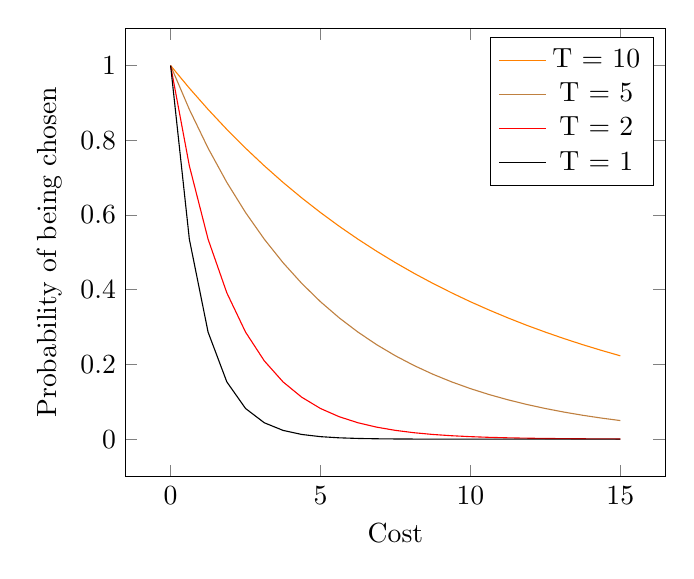
\begin{tikzpicture}
        \begin{axis}[
            xlabel = Cost,
            ylabel = Probability of being chosen
        ]
        \addplot[
            color=orange,
            domain=0:15
        ]
        {exp(-x / 10)};
        \addlegendentry{T = 10}
        \addplot[
            color=brown,
            domain=0:15
        ]
        {exp(-x / 5)};
        \addlegendentry{T = 5}
        \addplot[
            color=red,
            domain=0:15
        ]
        {exp(-x / 2)};
        \addlegendentry{T = 2}
        \addplot[
            color=black,
            domain=0:15
        ]
        {exp(-x / 1)};
        \addlegendentry{T = 1}
        \end{axis}
    \end{tikzpicture}
\end{figure}

\textbf{Temperature, Cooling Rate, and Max Iterations}

The greater the number of cities, the larger the search space, and hence greater chance of being stuck in a location minimum.
As a result, the temperature needs to be higher, or the cooling rate lower.

ADD MORE
\\

\textbf{Local Search}

It is an important part of the algorithm to determine an algorithm to search for nearby possible solutions.
A well known method is the \textbf{two-opt} method.
This involves selecting two random cities, re-orders the route between each other so that it does not.
\\

The example below shows before (on the left), and after reversing the order between nodes B and E (on the right).

\begin{figure}[!h]
    \centering
    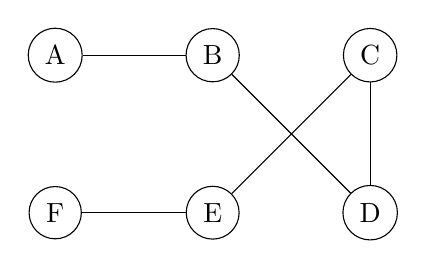
\begin{tikzpicture}
        \node[shape=circle,draw=black] (A) at (0,2) {A};
        \node[shape=circle,draw=black] (B) at (2,2) {B};
        \node[shape=circle,draw=black] (C) at (4,2) {C};
        \node[shape=circle,draw=black] (D) at (4,0) {D};
        \node[shape=circle,draw=black] (E) at (2,0) {E};
        \node[shape=circle,draw=black] (F) at (0,0) {F};
    
        \path [-](A) edge node[left] {} (B);
        \path [-](B) edge node[left] {} (D);
        \path [-](D) edge node[left] {} (C);
        \path [-](C) edge node[left] {} (E);
        \path [-](E) edge node[left] {} (F);
    \end{tikzpicture}
    \quad \quad \quad
    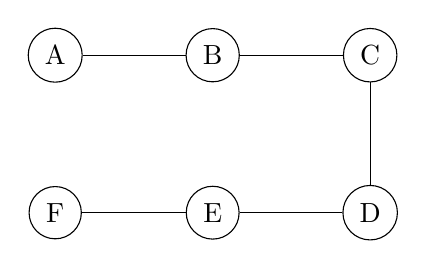
\begin{tikzpicture}
        \node[shape=circle,draw=black] (A) at (0,2) {A};
        \node[shape=circle,draw=black] (B) at (2,2) {B};
        \node[shape=circle,draw=black] (C) at (4,2) {C};
        \node[shape=circle,draw=black] (D) at (4,0) {D};
        \node[shape=circle,draw=black] (E) at (2,0) {E};
        \node[shape=circle,draw=black] (F) at (0,0) {F};
    
        \path [-](A) edge node[left] {} (B);
        \path [-](B) edge node[left] {} (C);
        \path [-](C) edge node[left] {} (D);
        \path [-](D) edge node[left] {} (E);
        \path [-](E) edge node[left] {} (F);
    \end{tikzpicture}
\end{figure}

Note that the one of the most modern methods is the LKH (Lin–Kernighan heuristic), however, this is a variation of the two-opt and three-opt method.

\end{document}
